\documentclass[a4paper]{article}
\usepackage[utf8]{inputenc}
\usepackage[T1]{fontenc}
\usepackage[francais]{babel}
\usepackage{fancyhdr}
\usepackage{lastpage}
\usepackage[left=2cm,right=2cm,top=2cm,bottom=4cm]{geometry}
\usepackage{scalerel}
\usepackage{enumerate}
\usepackage{xcolor}
\usepackage{listings}
\usepackage{xspace}
\usepackage{url}
\usepackage{lmodern}
\usepackage{float}
\usepackage{todonotes}
\usepackage{multirow}
\usepackage{subcaption}
\usepackage{caption}

\definecolor{myblue}{rgb}{0.33,0.61,0.83}
\definecolor{mygreen}{rgb}{0.39,0.56,0.31}
\definecolor{myorange}{rgb}{0.80,0.56,0.47}

\lstset{
	basicstyle=\ttfamily,
	backgroundcolor=\color{gray!10!white},
	xleftmargin=6pt,
	framexleftmargin=6pt,
	xrightmargin=6pt,
	framexrightmargin=6pt,
	framextopmargin=6pt,
	framexbottommargin=6pt,
	frame=tb,
	framerule=0pt,
	columns=fullflexible,
	breaklines=true,
	tabsize=2,
	%commentstyle=\color{mygreen},
	%keywordstyle=\color{myblue},
	%stringstyle=\color{myorange}
}

\setlength{\headheight}{50pt}
\setlength\parindent{0pt}

\lhead{
\includegraphics[scale=0.8]{imgs/logo-mse.png} \vspace{8pt}}

\rhead{\textbf{Data Mining en utilisant RapidMiner} \\
Romain Claret, Dorian Magnin \& Damien Rochat \\
Web Mining 2019}

\cfoot{Page \thepage\ / \pageref{LastPage}}

\pagestyle{fancy}

\begin{document}

\part*{Application de techniques de Data Mining en utilisant le logiciel RapidMiner}
Ce laboratoire a pour objectif d'expérimenter un logiciel de Data Mining, à savoir RapidMiner.
Celui-ci va nous permettre de mettre en place rapidement et simplement diverses tâches de prétraitement, d'appliquer des algorithmes de classification, de clustering, etc. et d'évaluer les résultats obtenus.

\section{Classification de spams}
Ci-dessous, la matrice de confusion résultant de la classification des SMS, avec le classificateur \textit{Naive Bayes}.
\begin{table}[H]
	\centering
	\def\arraystretch{2.0}
	\begin{tabular}{cccl}
	& \textbf{}
	& \multicolumn{2}{c}{\textbf{Prédiction}}\\\cline{3-4} 
	& \multicolumn{1}{c|}{}
	& \multicolumn{1}{c|}{\textbf{Spam}}
	& \multicolumn{1}{c|}{\textbf{Non-spam}}\\ \cline{2-4} 
	\multicolumn{1}{c|}{\multirow{2}{*}{\textbf{Vérité}}}
	& \multicolumn{1}{c|}{\textbf{Spam}}
	&\multicolumn{1}{c|}{92}
	& \multicolumn{1}{c|}{3}\\ \cline{2-4} 
	\multicolumn{1}{c|}{}
	& \multicolumn{1}{c|}{\textbf{Non-spam}}
	& \multicolumn{1}{c|}{38}
	& \multicolumn{1}{c|}{263}\\ \cline{2-4} 
	\end{tabular}
	\caption{Classification des SMS avec un filtrage Bayesien.}
\end{table}
Ce qui donne une accuracy de \textbf{89.65\%}.

\subsubsection*{Dans le bloc "Process Documents from Data" nous n'avons pas mis d'étape de stemming. Est-ce que l'ajout de ce préprocessing a un impact sur les résultats obtenus ?}
Une étape de Stemming Porter (algorithme adapté à la langue anglaise) a été ajoutée après le filtrage des stopwords.
Ceci ne change quasiment pas les résultats obtenus, comme le montre la matrice de confusion suivante :
\begin{table}[H]
	\centering
	\def\arraystretch{2.0}
	\begin{tabular}{cccl}
	& \textbf{}
	& \multicolumn{2}{c}{\textbf{Prédiction}}\\ \cline{3-4} 
	& \multicolumn{1}{c|}{}
	& \multicolumn{1}{c|}{\textbf{Spam}}
	& \multicolumn{1}{c|}{\textbf{Non-spam}} \\ \cline{2-4} 
	\multicolumn{1}{c|}{\multirow{2}{*}{\textbf{Vérité}}}
	& \multicolumn{1}{c|}{\textbf{Spam}}
	& \multicolumn{1}{c|}{91}
	& \multicolumn{1}{c|}{4}\\ \cline{2-4} 
	\multicolumn{1}{c|}{}
	& \multicolumn{1}{c|}{\textbf{Non-spam}}
	& \multicolumn{1}{c|}{38}
	& \multicolumn{1}{c|}{263}               \\ \cline{2-4} 
	\end{tabular}
	\caption{Classification des SMS avec Naive Bayes et Stemming.}
\end{table}

Cette nouvelle étape amène juste le système à se tromper sur un SMS en ne le classant pas comme spam, ajoutant donc un Faux Négatif.

\subsubsection*{Dans l'exemple ci-dessus, nous avons utilisé un classificateur bayésien, veuillez essayer d'autres familles de classificateurs, quel est l'impact sur le résultat obtenu ?}

Tout d'abord, un \textit{Arbre de décision} va avoir une excellente précision lorsqu'il va prédire un SMS comme étant un spam, il ne fait aucune erreur dans ce cas là.
En revanche, il laisse passer beaucoup de spams en ne les détectant pas.


\begin{table}[H]
	\centering
	\def\arraystretch{2.0}
	\begin{tabular}{cccl}
	& \textbf{}
	& \multicolumn{2}{c}{\textbf{Prédiction}}\\ \cline{3-4}
	& \multicolumn{1}{c|}{}
	& \multicolumn{1}{c|}{\textbf{Spam}}
	& \multicolumn{1}{c|}{\textbf{Non-spam}} \\ \cline{2-4} 
	\multicolumn{1}{c|}{\multirow{2}{*}{\textbf{Vérité}}}
	& \multicolumn{1}{c|}{\textbf{Spam}}
	& \multicolumn{1}{c|}{71}
	& \multicolumn{1}{c|}{24}\\ \cline{2-4} 
	\multicolumn{1}{c|}{}
	& \multicolumn{1}{c|}{\textbf{Non-spam}}
	& \multicolumn{1}{c|}{0}
	& \multicolumn{1}{c|}{301}\\ \cline{2-4} 
	\end{tabular}
	\caption{Classification des SMS avec un arbre de décision.}
\end{table}

Malgré tout, l'arbre de décision permet d'arriver à une accuracy de \textbf{93.94\%}, ce qui est sensiblement meilleur qu'un filtrage bayésien.
\\

Nous avons ensuite changé le classificateur pour un \textit{Réseau de neurones}.

\begin{table}[H]
	\centering
	\begin{tabular}{cccl}
	\def\arraystretch{2.0}
	& \textbf{}
	& \multicolumn{2}{c}{\textbf{Prédiction}}\\ \cline{3-4}
	& \multicolumn{1}{c|}{}
	& \multicolumn{1}{c|}{\textbf{Spam}}
	& \multicolumn{1}{c|}{\textbf{Non-spam}} \\ \cline{2-4} 
	\multicolumn{1}{c|}{\multirow{2}{*}{\textbf{Vérité}}}
	& \multicolumn{1}{c|}{\textbf{Spam}}
	& \multicolumn{1}{c|}{88}
	& \multicolumn{1}{c|}{7}\\ \cline{2-4} 
	\multicolumn{1}{c|}{}
	& \multicolumn{1}{c|}{\textbf{Non-spam}}
	& \multicolumn{1}{c|}{4}
	& \multicolumn{1}{c|}{297}\\ \cline{2-4} 
	\end{tabular}
	\caption{Classification des SMS avec un réseau de neurones.}
\end{table}

En ne commettant que 11 erreurs, sur 396 SMS, le réseau de neurones arrive à la meilleure accuracy parmis les classificateurs testés, à savoir \textbf{97.22\%}.

\subsubsection*{Finalement, vous utiliserez la seconde source de données (emails.zip) sur laquelle vous appliquerez le même process. Que constatez-vous en comparant les 2 résultats ?}

Nous avons au préalable eu à préprocesser les données des emails. Dans RapidMiner, nous avons ajouté un bloc permettant de transformer la colonne « spam » en type binomiale et de lui définir le rôle de label (blocs \textit{Numerical to Binomial} et \textit{Set Role}).
\\
De plus, le contenu de la colonne avec le contenu des emails a été tronqué de " Subject : ". Ceci n'affecte évidemment pas le résultat, car il est présent dans chaque élément et n'est donc pas relevant et est ignoré par les algorithmes. Mais ce traitement permet de rendre le modèle réutilisable.
\\\\
Avec un classificateur \textit{Naive Bayes}, nous arrivons à la matrice de confusion suivante :


\begin{table}[H]
	\centering
	\begin{tabular}{cccl}
	\def\arraystretch{2.0}
	& \textbf{}
	& \multicolumn{2}{c}{\textbf{Prédiction}}\\ \cline{3-4}
	& \multicolumn{1}{c|}{}
	& \multicolumn{1}{c|}{\textbf{Spam}}
	& \multicolumn{1}{c|}{\textbf{Non-spam}} \\ \cline{2-4}
	\multicolumn{1}{c|}{\multirow{2}{*}{\textbf{Vérité}}}
	& \multicolumn{1}{c|}{\textbf{Spam}}
	& \multicolumn{1}{c|}{340}
	& \multicolumn{1}{c|}{11}\\ \cline{2-4} 
	\multicolumn{1}{c|}{}
	& \multicolumn{1}{c|}{\textbf{Non-spam}}
	& \multicolumn{1}{c|}{38}
	& \multicolumn{1}{c|}{1249}\\ \cline{2-4} 
	
	\end{tabular}
	\caption{Classification des emails avec un filtrage Bayesien.}
\end{table}

Avec une accuracy de \textbf{97.01\%}, il s'agit d'un très bon résultat.
Ajouter une étape de stemming n'améliore pas non plus le résultat sur ce type de données.
\\

Nous avons également essayé d'utiliser un arbre de décision avec les emails.
Celui-ci nous a permis d'arriver à une accuracy de \textbf{86.81\%}, avec beaucoup de Faux Négatifs, ce qui est bien moins efficace.
Un arbre de décision est de moins en moins efficace plus la taille et la complexité des données augmentent.

\begin{table}[H]
	\centering
	\begin{tabular}{cccl}
	\def\arraystretch{2.0}
	& \textbf{}
	& \multicolumn{2}{c}{\textbf{Prédiction}}\\ \cline{3-4} 
	& \multicolumn{1}{c|}{}
	& \multicolumn{1}{c|}{\textbf{Spam}}
	& \multicolumn{1}{c|}{\textbf{Non-spam}} \\ \cline{2-4} 
	\multicolumn{1}{c|}{\multirow{2}{*}{\textbf{Vérité}}}
	& \multicolumn{1}{c|}{\textbf{Spam}}
	& \multicolumn{1}{c|}{166}
	& \multicolumn{1}{c|}{212}\\ \cline{2-4} 
	\multicolumn{1}{c|}{}
	& \multicolumn{1}{c|}{\textbf{Non-spam}} & \multicolumn{1}{c|}{4}
	& \multicolumn{1}{c|}{1256}\\ \cline{2-4} 
	\end{tabular}
	\caption{Classification des emails avec un arbre de décision.}
\end{table}


\pagebreak
\section{Market basket analysis}

\subsection{Details sur l'implémentation et ses résultats}
Pour la création des fichiers CSV utilisés pour la génération de règles d'associations, un nettoyage des données a été fait.
\\
Les lignes avec des données vides, comme par exemple le nom du produit sont filtrées.
Il en est de même si la quantité est plus petite que 0.
Un programme a été implémenté afin de détecter et filtrer les lignes avec des éventuels noms de produit incohérents.
\\\\
Voici une liste des noms incohérents trouvés :
\textit{wet pallet,sold in set?,wet damaged,faulty,posy candy bag,michel oops,wet/mouldy,
lost,dagamed,daisy notebook,fba,taig adjust,water damage,ribbons purse,?display?,found in w/hse,damaged stock,
samples,
mixed up,
???missing,breakages,chilli lights,dotcom set,re-adjustment, packing charge,amazon sales,?,
mix up with c,owl doorstop,stock check,mia,wrap folk art,carriage,damages,?lost,john lewis,found box,20713,show samples,damages wax,website fixed,jumbo bag owls,wet boxes,frog candle,found,given away,mouldy,???,broken,
wrong code,damages?,display,wet,bunny egg box,polkadot pen,?missing,dotcom,amazon adjust,damaged,returned,
toybox  wrap,smashed,?sold as sets?,showroom,led tea lights,wet/rusty,missing?,wrong barcode,lost in space,
crushed ctn,popcorn holder,dotcom sales,lost??,sold as 1,bingo set,thrown away.,crushed boxes,test,check,crushed,
wet?,mailout,amazon,rain poncho,adjust,ebay,adjustment,spotty bunting,wet rusty,
cracked,
sale error,???lost,
water damaged,missing,garage key fob,dotcomstock,dotcom adjust,sold as 22467,??,dotcom postage,jumbo bag toys,
shoe shine box,?? missing,on cargo order,wrong code?,check?,label mix up,postage,
wrap carousel,can't find,wrongly marked,retrospot lamp,thrown away,counted,????missing,cordial jug}
\\\\
De plus, chaque donnée de colonne est systématiquement trimée pour éviter tout problème et pour faciliter la suite du traitement. 
Voici quelques statistiques calculées lors du filtrage :
\\

\begin{itemize}
	\item Nombre de lignes dans le fichier : 541'909
	\item Nombre de lignes après nettoyage : 397'924
	\item Nombre de produits : 3'639
\end{itemize}

\vspace{6pt}
Le programme a donc retiré 143'985 lignes.
\\\\
Un autre programme a été implémenté pour standardiser la description des produits en la liant avec le numéro du produit et celle qui est la plus utilisée, dans le cas un produit aurait plusieurs descriptions. \\
Pour voir une partie de l'algorithme, il faut regarder la fonction \textit{Main.resolveProductDescription()} dans le code Java fourni en annexe.
\\\\
Ci-dessous, d'autres informations que nous calculons lors de la création des nouveaux fichiers CSV.
\\\\
Création du fichier par pays (permets de tester rapidement le code) :
\begin{itemize}
	\item Nombre de lignes dans le nouveau fichier byCountry.csv : 37
	\item Durée du traitement: 00:01.625
\end{itemize}
\vspace{6pt}

Création du fichier par client :
\begin{itemize}
	\item Nombre de lignes dans le nouveau fichier byCustomer.csv : 4'339
	\item Durée du traitement: 01:44.361
\end{itemize}

\vspace{6pt}

Création du fichier par facture :
\begin{itemize}
	\item Nombre de lignes dans le nouveau fichier byInvoice.csv : 18'536
	\item Durée du traitement: 07:26.901
\end{itemize}

\vspace{6pt}

Afin de pouvoir générer ces données, nous avons utilisé du multi-threading ce qui nous a permis d'améliorer considérablement le temps nécessaire à la création des fichiers.
\\\\
Pour lire le fichier, nous avons dû en créer un nouveau et copiant et collant son contenu. Nous pensons qu'il doit y avoir un problème d'encodage. 
\\\\
Pour tester le programme, il suffit de lancer la commande \textit{mvn clean install}, de modifier le fichier \textit{application.properties} avec l'emplacement des fichiers de base et de destination.
\\\\
La création de ces fichiers n'est pas simple et nous a pris beaucoup de temps. Par exemple, nous pourrions encore améliorer la génération, en tenant compte des produits retournés.
Il serait aussi bien d'avoir un meilleur descriptif de ces données.
\\\\
Nous avons ensuite utilisé ces différents sets de données dans RapidMiner.
\\
Le process créé se charge de définir la colonne ID comme étant l'identifiant à utiliser pour la suite et de convertir les booléens de la matrice en valeurs binomiales.
\\\\
Ensuite, le bloc \textit{FP-Growth} se charge de compter la fréquence des différents achats. Il utilise le format d'input \textit{items in dummy coded columns} qui correspond à la matrice de booléens contenue dans les fichiers.
\\\\
Finalement, le dernier bloc génère les règles d'associations.

\begin{figure}[H]
	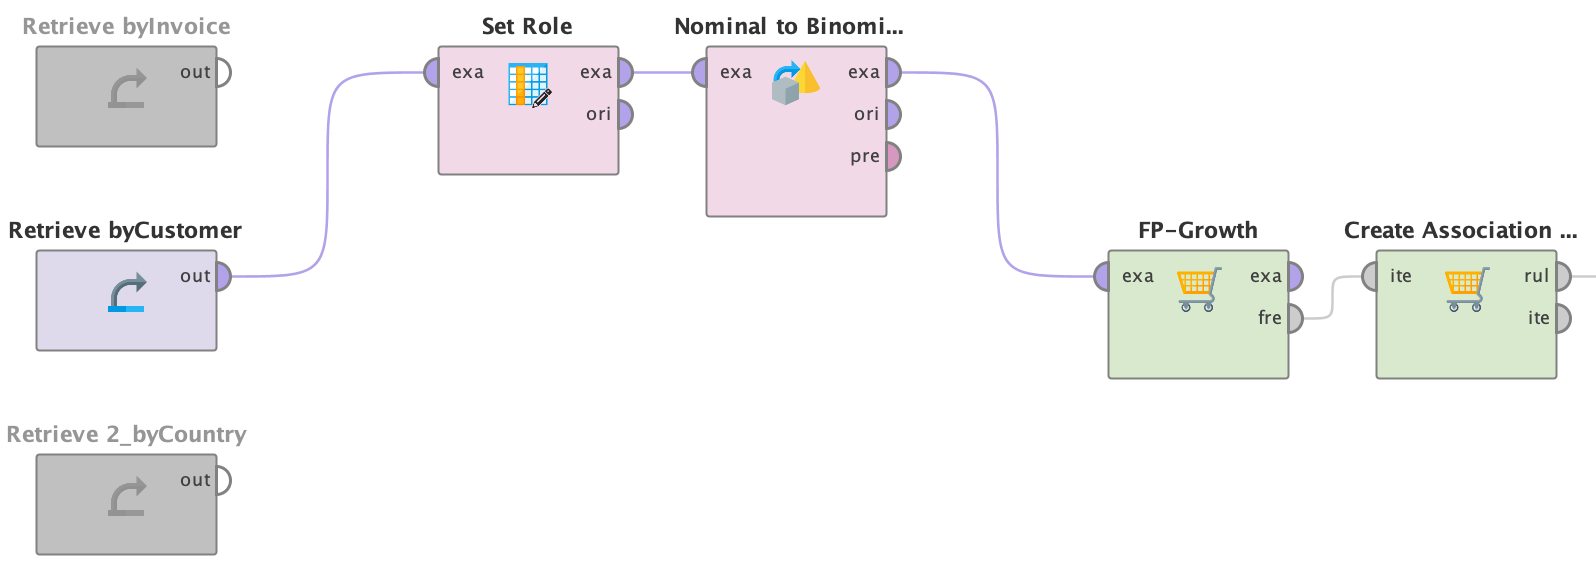
\includegraphics[width=\linewidth]{imgs/part_2/2_full_process_1}
	\caption{Process 2: Market Basket with boolean matrix}
	\label{fig:2_full_process_1}
\end{figure}

Nous avons également essayé une autre méthode pour fournir les données au \textit{FP-Growth}, en effet il en existe 2 de plus de la méthode mentionnée ci-dessus. Ici nous avons exploré la méthode de la concaténation. Mais il existe également la méthode de la liste espèce de liste.
\\\\
La méthodologie est la suivante:
\begin{itemize}
	\item Nous utilisons le module d'agrégation pour concaténer notre champ \textit{Description} et le grouper par l'attribue \textit{InvoiceNo}.
	\item Nous renommons ensuite notre nouvelle colonne en \textit{Produit} dans un but esthétique.
	\item Nous définition une d'\textit{id} à notre attribut de groupage \textit{InvoiceNo}
	\item Puis nous utilisons l'option \textit{item list in a column} pour notre \textit{FP-Growth} en gardant les paramètres par défaut.
	\item Puis finalement, utilisons le module \textit{Create Association} avec ses paramètres par défauts.
\end{itemize}

\vspace{6pt}

Nous avons pu faire fonctionner que le "par facture", dans un temps quasi instantané. Les résultats nous semblent corrects. (Figs.\ref{fig:2_process_2_results_freq},\ref{fig:2_process_2_results_1_assoc_1},\ref{fig:2_process_2_results_1_assoc_2}) Cependant, pour "par clients", il en résulte en un échec dû à un manque de RAM (Fig,\ref{fig:2_fail}). 
\\\\
De plus, nos fichiers générés \textit{byInvoice.csv} et \textit{byCustomer.csv} contiennent une grande quantité de données et nous nous sommes malheureusement heurtés à des problèmes matériels durant l'exécution de ce process également. En plus d'être extrêmement long, ce processus n'a jamais été capable de se terminer avec succès, car RapidMiner arrivait sans cesse à court de mémoire RAM.(Fig.\ref{fig:2_fail})
\\
Nous n'avons donc pas eu la chance d'obtenir de résultat à cette étape.
\\\\
Pour finir, nous somme tout à fait conscient de la raison logique qui implique que le calcule nécessaire pour effectuer "par facture" est moindre par rapport au "par client". En effet, nous avons un set de \textbf{25900} IDs uniques pour les factures et \textbf{139452} IDs uniques pour les clients, soit plus de 5 fois plus, avec une répercussion matricielle.
\\\\
Les valeurs ont été extraite à l'aide d'un script python.
\begin{lstlisting}[language=python]
>>> import pandas
>>> data = pandas.read_csv('data.csv')
>>> print("invoices count:",len(set(data['InvoiceNo'])))
>>> print("customers count:",len(set(data['CustomerID'])))
invoices count: 25900
customers count: 139452
\end{lstlisting}

\begin{figure}[H]
	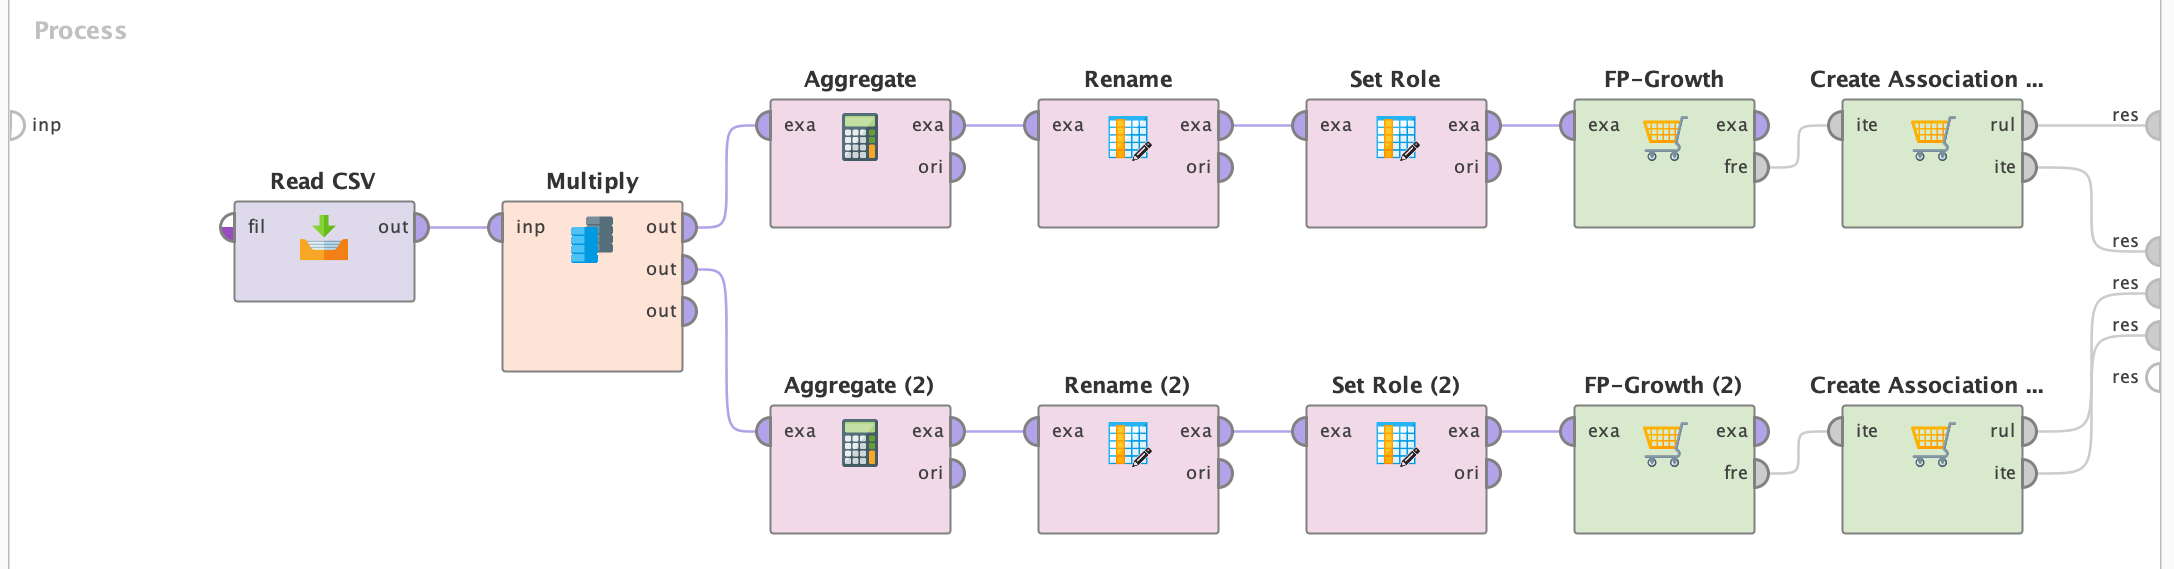
\includegraphics[width=\linewidth]{imgs/part_2/2_full_process_2}
	\caption{Process 2: Market Basket with concatenated columns}
	\label{fig:2_full_process_2}
\end{figure}

\begin{figure}[H]
	\centering
	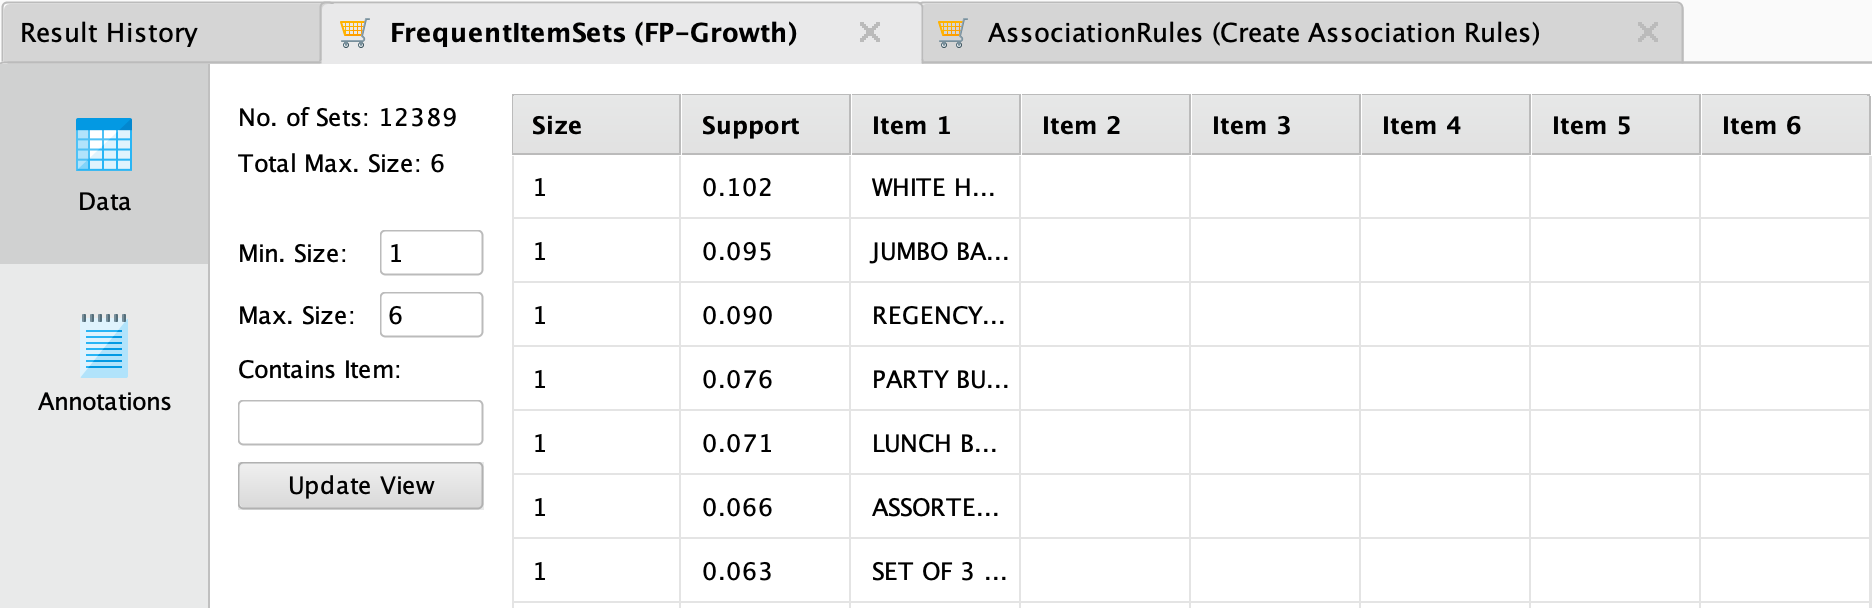
\includegraphics[width=\linewidth/1]{imgs/part_2/2_process_2_results_freq}
	\caption{Process 2 result: Frequencies}
	\label{fig:2_process_2_results_freq}
\end{figure}

\begin{figure}[H]
	\centering
	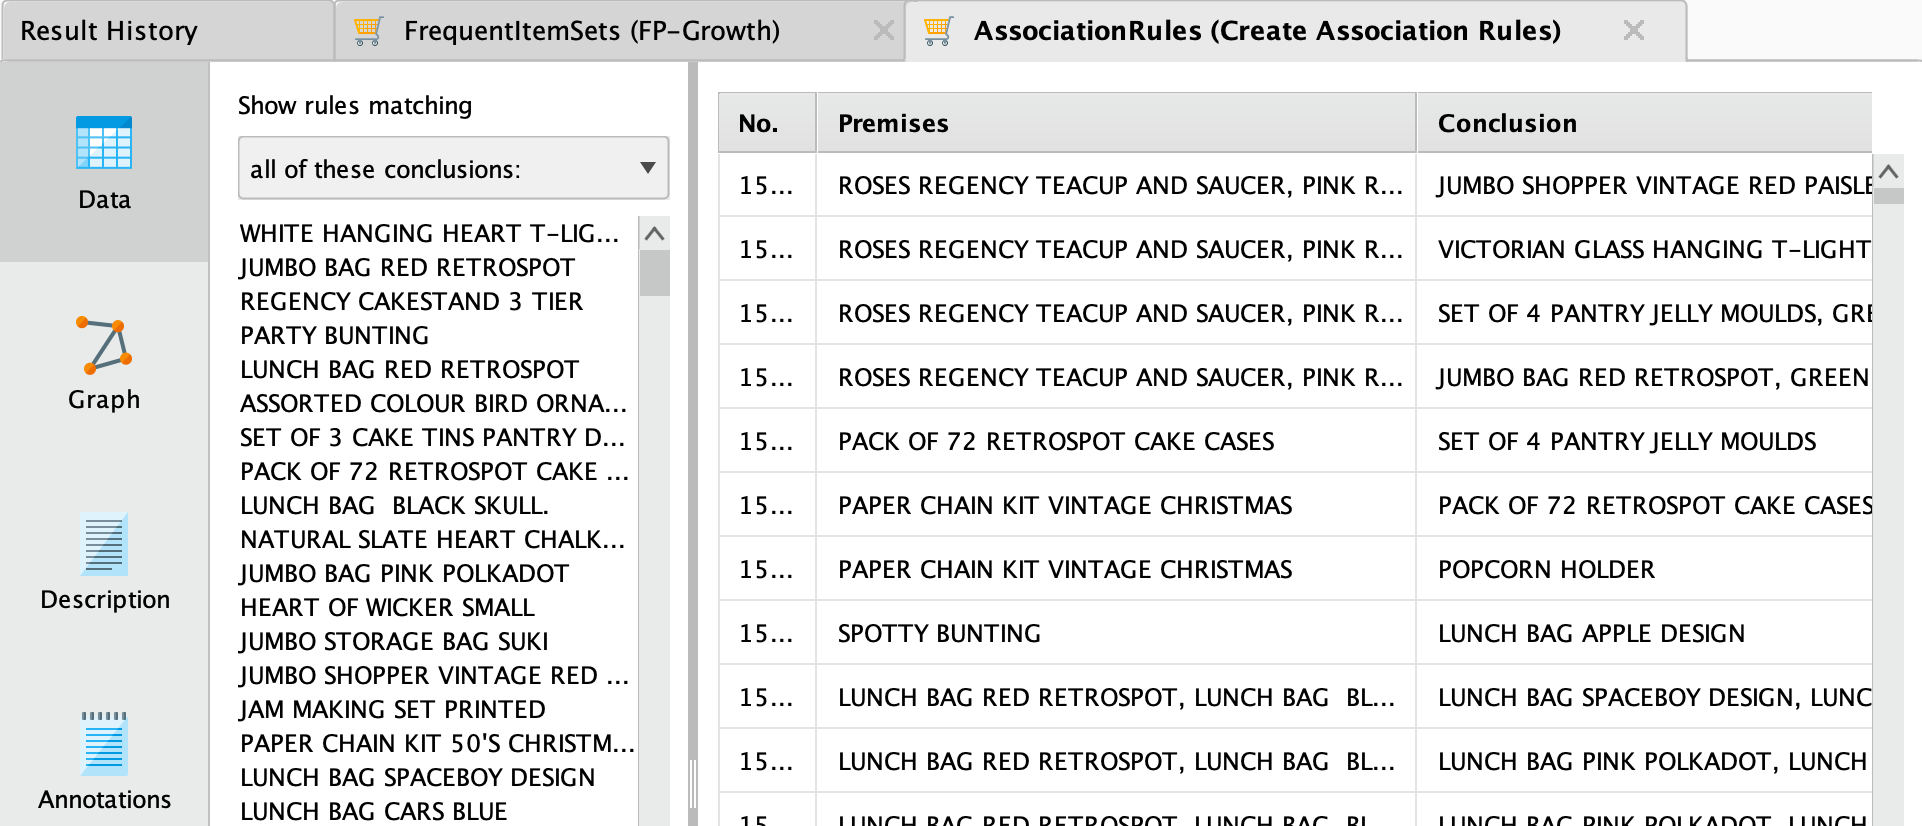
\includegraphics[width=\linewidth/1]{imgs/part_2/2_process_2_results_1_assoc_1}
	\caption{Process 2 result: Association Rule Part 1}
	\label{fig:2_process_2_results_1_assoc_1}
\end{figure}

\begin{figure}[H]
	\centering
	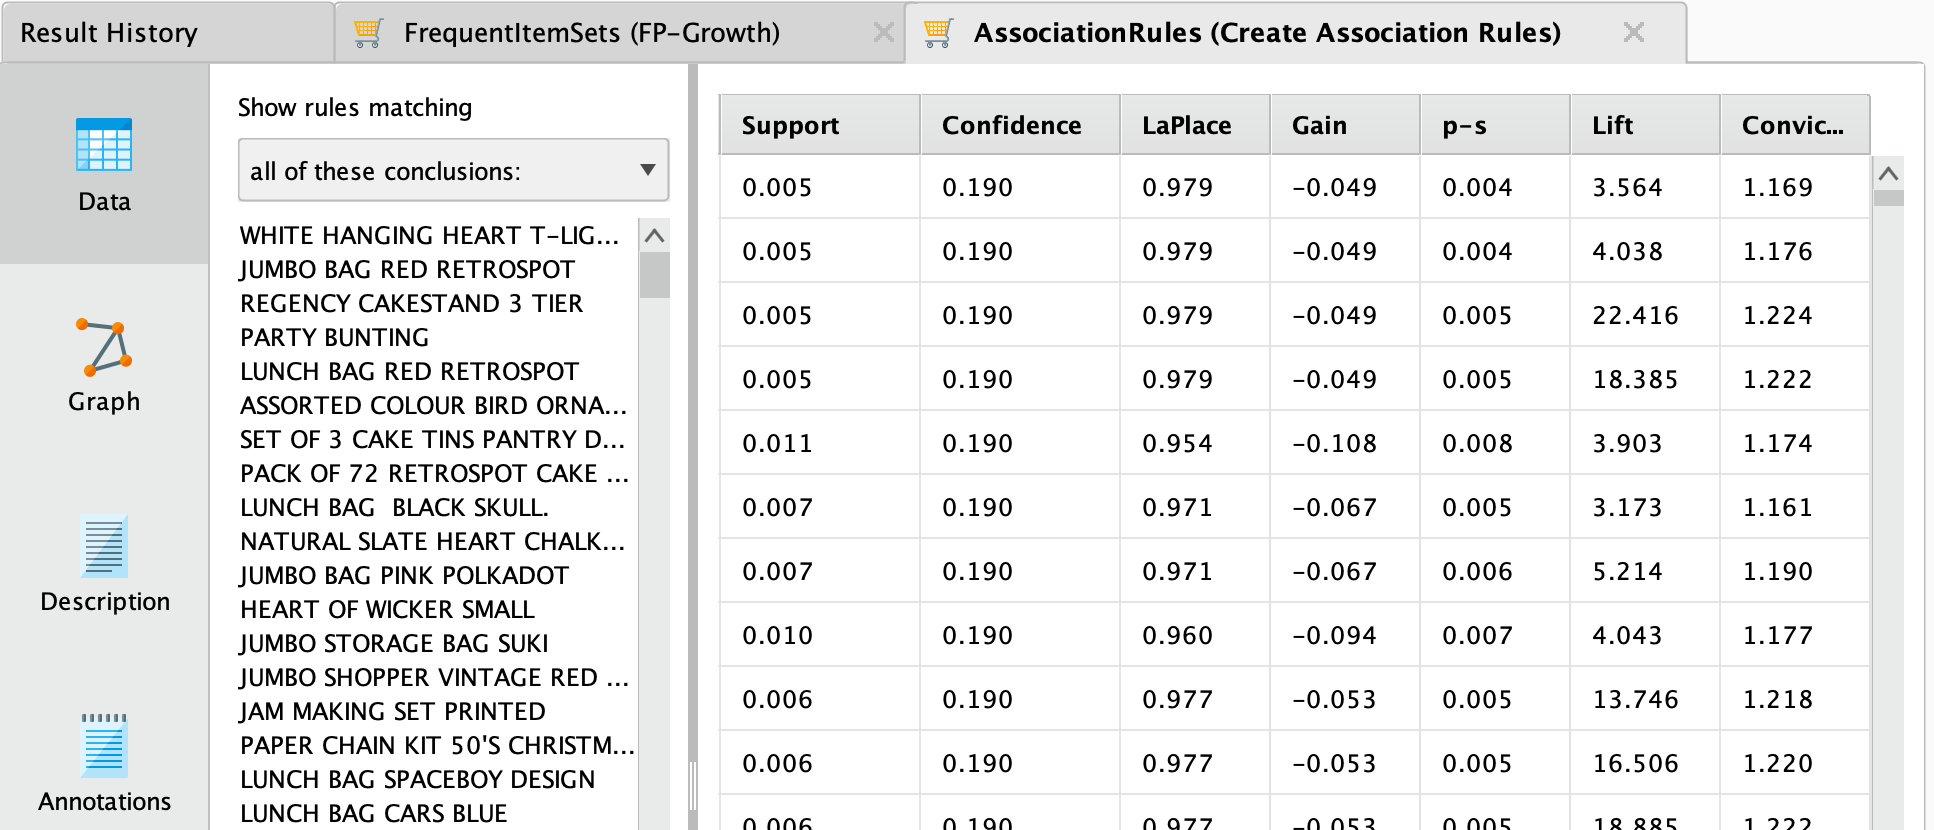
\includegraphics[width=\linewidth/1]{imgs/part_2/2_process_2_results_1_assoc_2}
	\caption{Process 2 result: Association Rule Part 2}
	\label{fig:2_process_2_results_1_assoc_2}
\end{figure}

\begin{figure}[H]
	\centering
	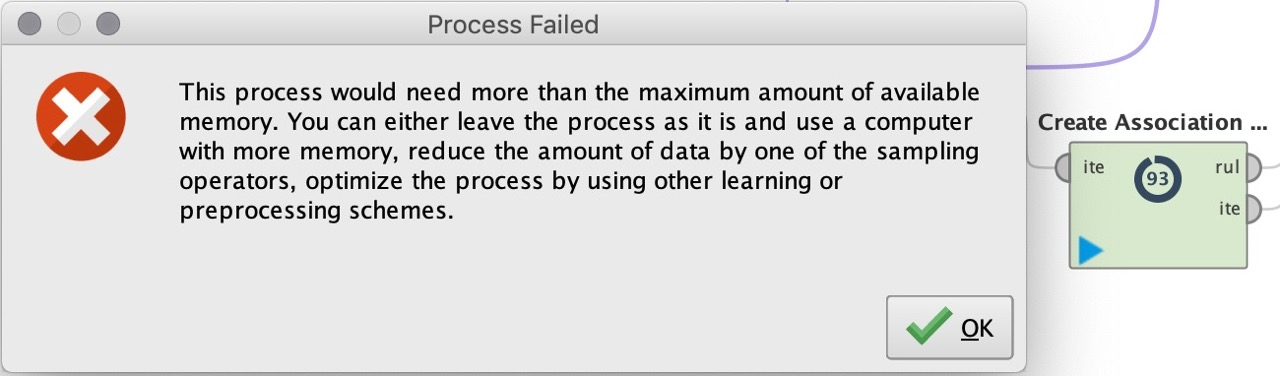
\includegraphics[width=\linewidth/1]{imgs/part_2/2_fail}
	\caption{Failure while creating association}
	\label{fig:2_fail}
\end{figure}

\vspace{6pt}

\pagebreak
\section{Utilisation d'un WordNet sur des commentaires d’utilisateurs}

\begin{figure}[H]
	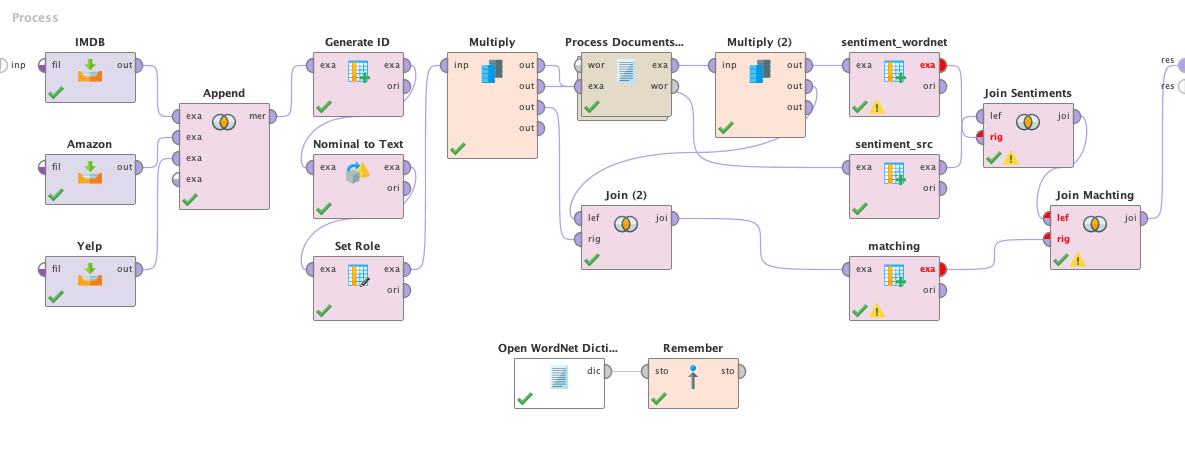
\includegraphics[width=\linewidth]{imgs/part_3/3_full_process}
	\caption{Processus complet: WordNet sur 3000 commentaires }
	\label{fig:3_full_process}
\end{figure}

Dans le cadre de cette 3e partie, nous avons mis en place un processus capable de comparer des commentaires sous format texte fourni avec un étiquetage du sentiment (Positif, Négatif, et Neutre), avec un algorithme de prédiction capable d'extraire le sentiment d'un texte basé sur le dictionnaire WordNet. Pour simplifier la comparaison, nous avons ajouté un attribue qui vérifie que le sentiment source est le même que le sentiment prédit (appelé chez nous matching).
\\\\
Nous allons pour ce faire prétraiter le texte fourni à l'aide de combinaisons de différentes techniques et fournir le résultat au module "Extract Sentiment de WordNet" qui générera une prédiction du sentiment lié à l'input.
\\\\
Nous utiliserons les modules suivants:
\begin{itemize}
	\item tokenisation
	\item transformation des caractères
	\item stopwords
	\item filtre sur la longueur des tokens
	\item stemming
\end{itemize}

\subsection{Questions sur les règles d'association}

\textbf{Commentez les résultats obtenus par rapport aux étiquettes existantes sur le dataset.}
\textbf{Quelle est l'influence des différentes étapes de "text processing" sur le résultat que vous obtenez ?}

\subsubsection{Module Extract Sentiment WordNet par défault}
Dans le but d'explorer les influences lié aux différentes étapes de "text processing" nous allons utiliser le module de WordNet qui permet d'extraire le sentiment d'input sous format texte avec ses paramètres par défaut. (Fig.\ref{fig:3_processing_documents_full_0_05}) (Nous verrons plus tard que la notion de texte sera faite sous forme de tokens, qui est une décomposition d'un texte en mots.)
\begin{figure}[H]
\centering
	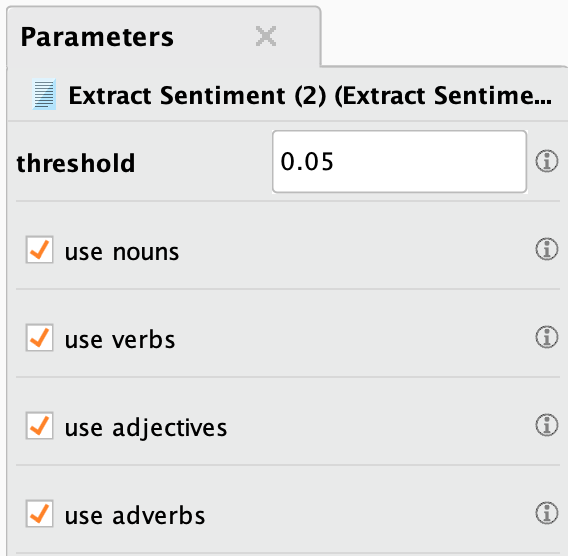
\includegraphics[width=\linewidth/3]{imgs/part_3/3_processing_documents_full_0_05}
	\caption{Extract Sentiment Default Threshold at 0.05}
	\label{fig:3_processing_documents_full_0_05}
\end{figure}


\vspace{6pt}
\subsubsection{Process Documents from Data uniquement avec le module d'extraction du sentiment WordNet}
Nous constatons un matching à \textbf{0\%}. En effet, le module "Extract Sentiment" n'est pas capable d'interpréter le texte brut des commentaires et par conséquent donne une sortie commune Neutre (basé sur la valeur numérique 0) à toutes les entrées.
\begin{figure}[H]
	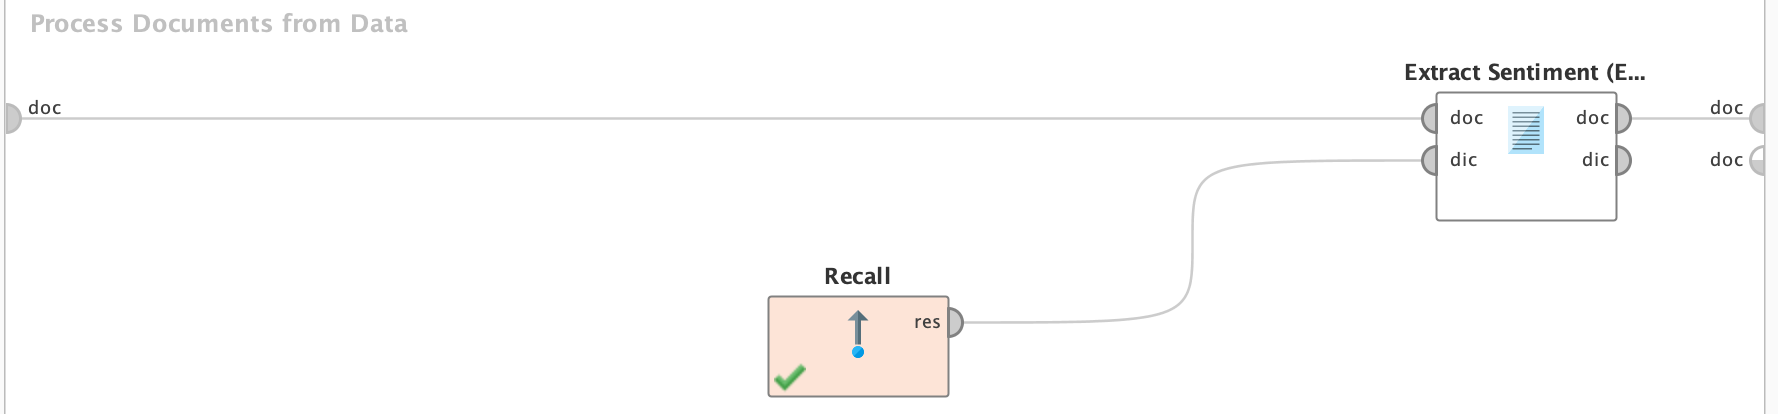
\includegraphics[width=\linewidth]{imgs/part_3/3_processing_documents_no_stem_filter_token_stopword_transform_tokens}
	\caption{Process Documents from Data with only the sentiment extractor from WordNet}
	\label{fig:3_processing_documents_no_stem_filter_token_stopword_transform_tokens}
\end{figure}
\begin{figure}[H]
	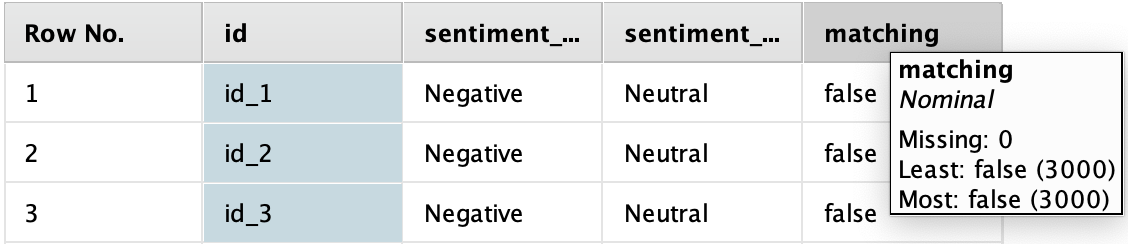
\includegraphics[width=\linewidth]{imgs/part_3/3_processing_documents_no_stem_filter_token_stopword_transform_tokens_results}
	\caption{Results of the Process Documents from Data with only the sentiment extractor from WordNet}
	\label{fig:3_processing_documents_no_stem_filter_token_stopword_transform_tokens_results}
\end{figure}

\vspace{6pt}
\subsubsection{Process Documents from Data composé de la tokenisation}
En utilisant la tokenisation avec son paramètre par défaut (non letters) le module "Extract Sentiment" a maintenant les ressources minimums pour fonctionner et permet une prédiction à \textbf{29.7\%}. (Fig.\ref{fig:3_processing_documents_no_stem_filter_token_stopword_transform_results})
\\
Il est intéressant de noter qu'il y a plusieurs options pour la tokenisation. En jouant avec ces paramètres, nous obtenons les résultats suivants: (notons: que nous cherchons à augmenter le nombre de matchs (true) de l'attribue matching)
\begin{itemize}
	\item non letters (par défaut): \textbf{70.3\%} (Fig.\ref{fig:3_processing_documents_no_stem_filter_token_stopword_transform_results})
	\item special characters (.:): \textbf{67.3\%}
	\item regular expression: Pas essayé
	\item linguistic sentences: \textbf{0\%}
	\item linguistic tokens: \textbf{69.8\%}
\end{itemize}
\vspace{6pt}

\begin{figure}[H]
	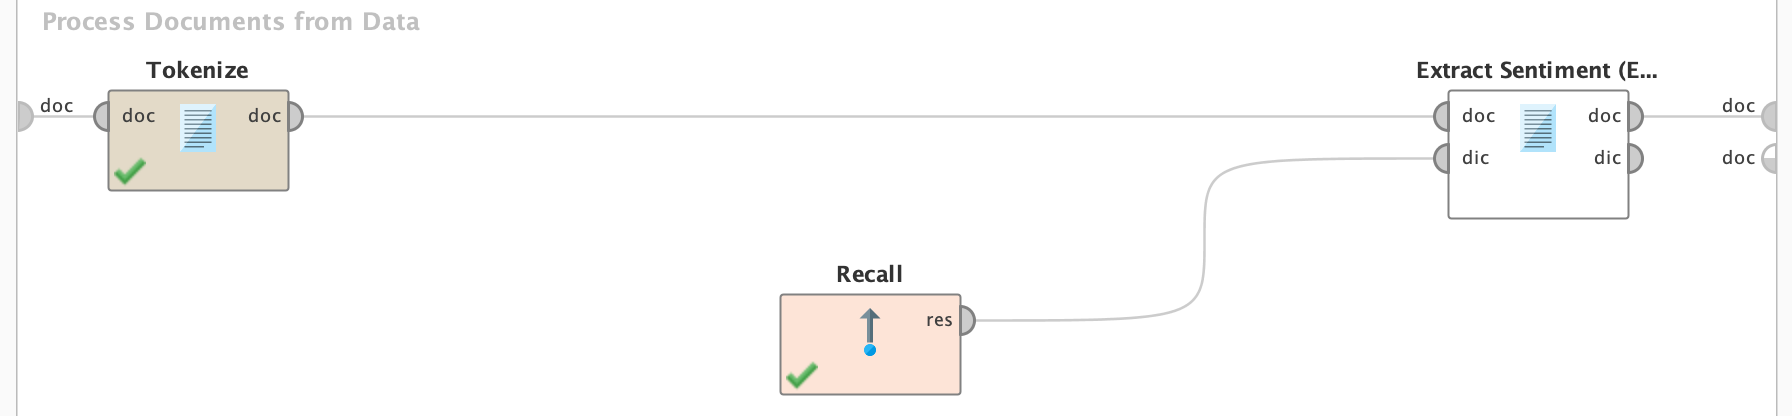
\includegraphics[width=\linewidth]{imgs/part_3/3_processing_documents_no_stem_filter_token_stopword_transform}
	\caption{Process Documents from Data with tokenization}
	\label{fig:3_processing_documents_no_stem_filter_token_stopword_transform}
\end{figure}
\begin{figure}[H]
	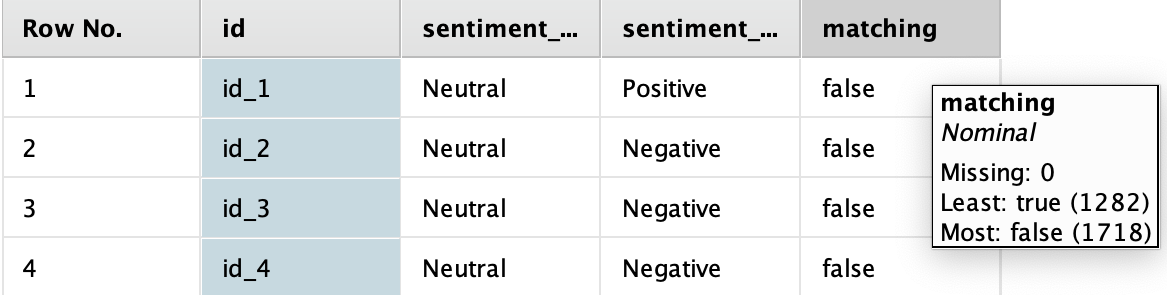
\includegraphics[width=\linewidth]{imgs/part_3/3_processing_documents_no_stem_filter_token_stopword_transform_results}
	\caption{Results of tokenization via non letters}
	\label{fig:3_processing_documents_no_stem_filter_token_stopword_transform_results}
\end{figure}

\vspace{6pt}
\subsubsection{Process Documents from Data composé de la tokenisation ainsi que de la transformation en caractères minuscules}
Nous ajoutons la transformation des tokens, en utilisant le paramètre par défaut: lower case. Nous avons également essayé la seconde option: upper case, cependant le résultat est le même. Ce module uniformise les lettres des tokens en soit minuscule ou minuscules. Ce traitement nous à fait perdre un match, cependant nous gardons notre \textbf{70.3\%}. Il est intéressant de constater que pour certains commentaires, l'effet de la capitalisation irrégulière puisse avoir un impact.
\begin{figure}[H]
	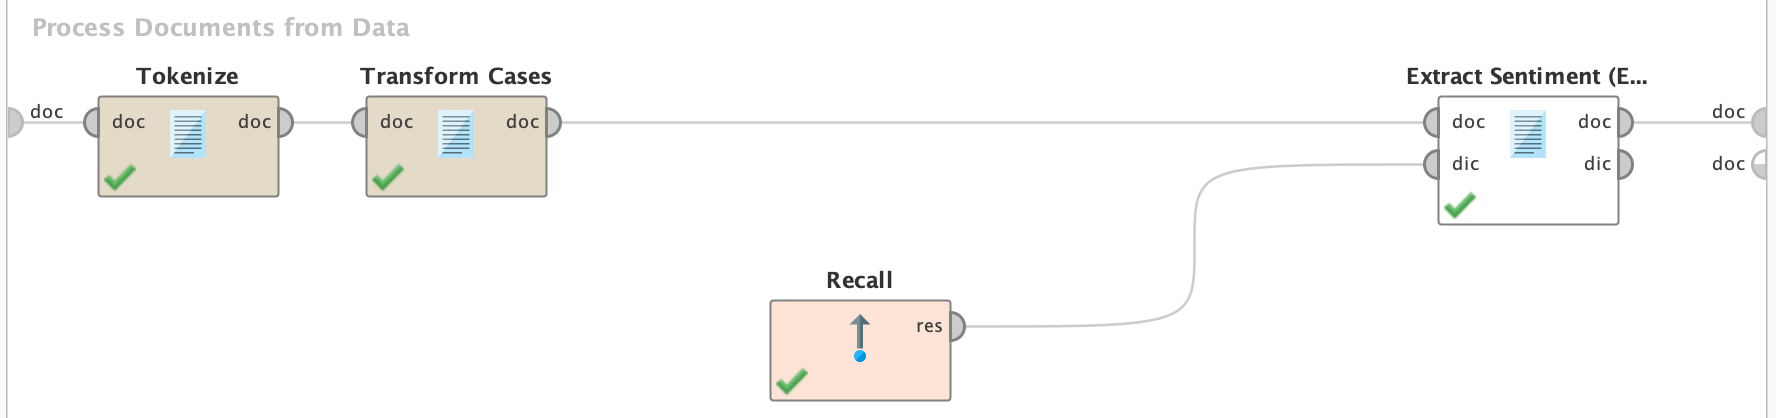
\includegraphics[width=\linewidth]{imgs/part_3/3_processing_documents_no_stem_filter_token_stopword}
	\caption{Process Documents from Data with tokenization and low character filter}
	\label{fig:3_processing_documents_no_stem_filter_token_stopword}
\end{figure}
\begin{figure}[H]
	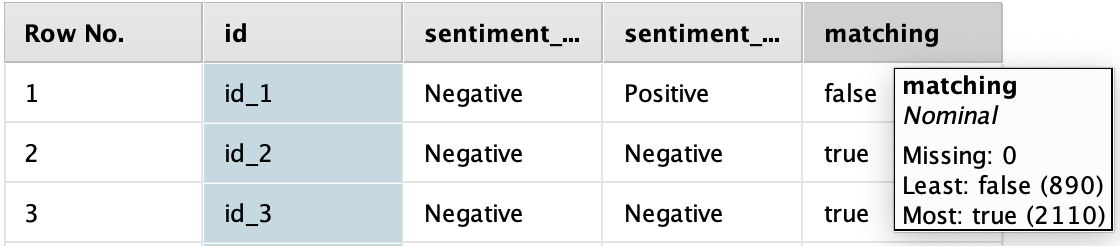
\includegraphics[width=\linewidth]{imgs/part_3/3_processing_documents_no_stem_filter_token_stopword_results}
	\caption{Results of the Process Documents from Data with tokenization and low character filter}
	\label{fig:3_processing_documents_no_stem_filter_token_stopword_results}
\end{figure}

\vspace{6pt}
\subsubsection{Process Documents from Data composé de la tokenisation, la transformation en caractères minuscules, et la suppression des stopwords}
En ajoutant le filtre des stopwords anglais. Nous constatons une perte en performance des prédictions avec \textbf{66.2\%}. Ce n'est pas le comportement que nous attendons généralement d'un filtre par stopword, au contraire. Nous pensons que cet effet est dû à la taille du corpus et de la perte du contexte lorsqu'il y a un sentiment fort, où l'utilisateur a tendance à accumuler via des mots de liaisons (inclue dans les stopwords) des adjectifs pour accentuer une opinion.
\begin{figure}[H]
	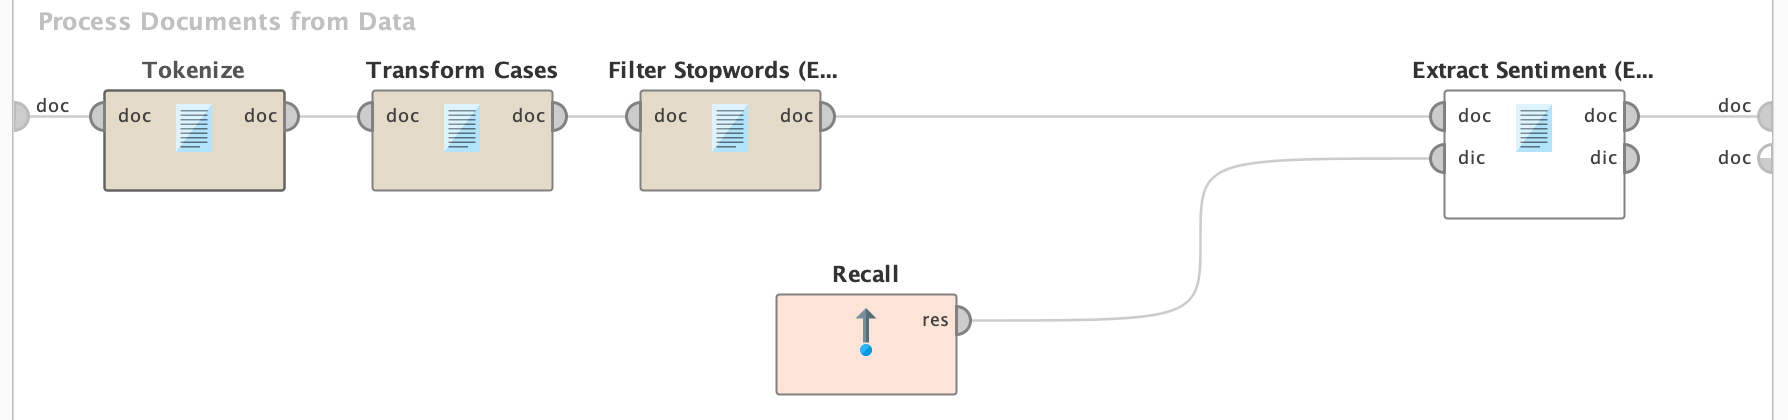
\includegraphics[width=\linewidth]{imgs/part_3/3_processing_documents_no_stem_filter_token}
	\caption{Process Documents from Data with the tokenizion, the low cases, and stopword filter}
	\label{fig:3_processing_documents_no_stem_filter_token}
\end{figure}
\begin{figure}[H]
	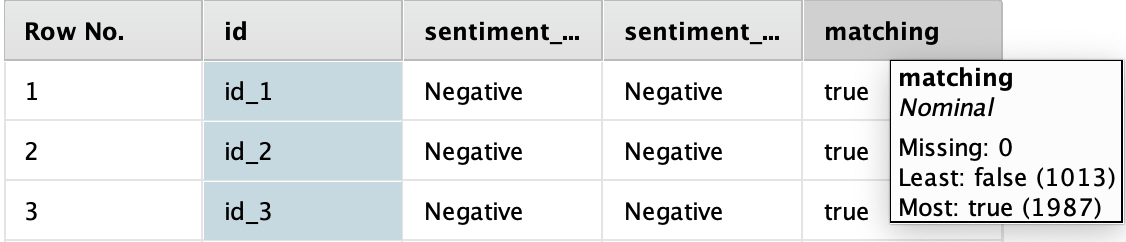
\includegraphics[width=\linewidth]{imgs/part_3/3_processing_documents_no_stem_filter_token_results}
	\caption{Results on the Process Documents from Data with the tokenizion, the low cases, and stopword filter}
	\label{fig:3_processing_documents_no_stem_filter_token_results}
\end{figure}

\vspace{6pt}
\subsubsection{Process Documents from Data composé de la tokenisation, la transformation en caractères minuscules, la suppression des stopwords, et un filtre sur la longueur des tokens}
En utilisant les paramètres par défauts (Fig.\ref{fig:3_processing_documents_filter_tokens_default_params}) nous obtenons une performance de \textbf{60.9\%}. Cependant en tweakant les paramètres (1 en taille minimum et en gardant la taille maximum par défault 14)(Fig.\ref{fig:3_processing_documents_filter_tokens_best_params}) nous arrivons à atteindre une performance de \textbf{66.3\%}.(Fig.\ref{fig:3_processing_documents_no_stem_best_results})

\begin{figure}[H]
	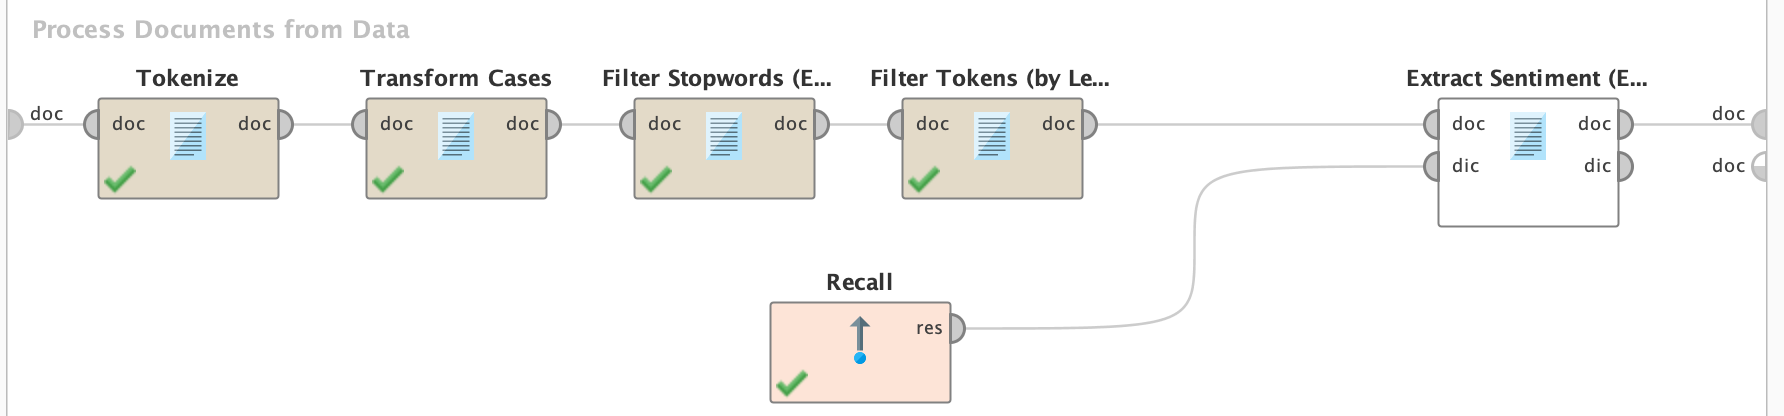
\includegraphics[width=\linewidth]{imgs/part_3/3_processing_documents_no_stem}
	\caption{Process Documents from Data with all elements expect stemming}
	\label{fig:3_processing_documents_no_stem}
\end{figure}
\begin{figure}[H]
	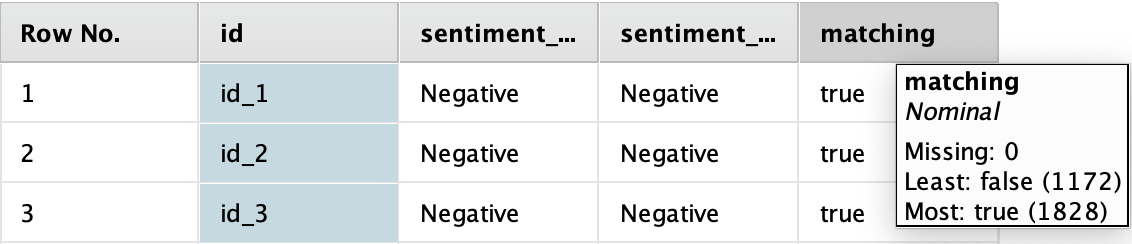
\includegraphics[width=\linewidth]{imgs/part_3/3_processing_documents_no_stem_results}
	\caption{Results for stemming with the defaults parameters}
	\label{fig:3_processing_documents_no_stem_results}
\end{figure}
\begin{figure}[H]
    \centering
    \begin{subfigure}[b]{0.4\textwidth}
        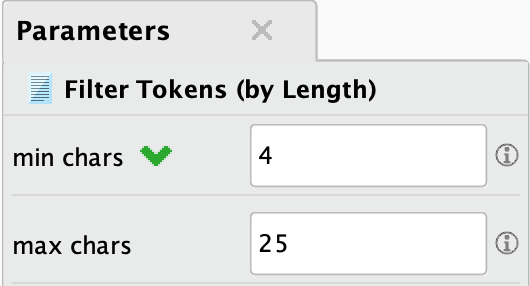
\includegraphics[width=\textwidth]{imgs/part_3/3_processing_documents_filter_tokens_default_params}
        \caption{Default parameters from the length filter}
        \label{fig:3_processing_documents_filter_tokens_default_params}
    \end{subfigure}
    \hspace{0.1\textwidth}
    \begin{subfigure}[b]{0.4\textwidth}
        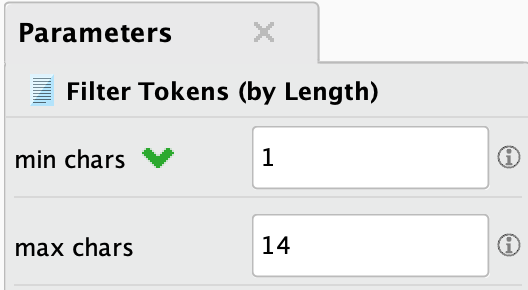
\includegraphics[width=\textwidth]{imgs/part_3/3_processing_documents_filter_tokens_best_params}
        \caption{Best parameters from the length filter}
        \label{fig:3_processing_documents_filter_tokens_best_params}
    \end{subfigure}
    \caption{Parameters from the length filter}
    \label{fig:3_processing_documents_filter_tokens_params}
\end{figure}

\begin{figure}[H]
	\centering
	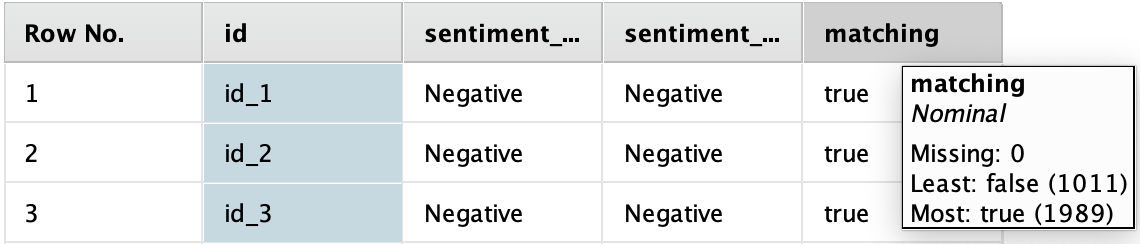
\includegraphics[width=\linewidth]{imgs/part_3/3_processing_documents_no_stem_best_results}
	\caption{Results of the best parameters from the length filter}
	\label{fig:3_processing_documents_no_stem_best_results}
\end{figure}


\vspace{6pt}
\subsubsection{Process Documents from Data en ajoutant le stemming}
Voir figure \ref{fig:3_processing_documents_full} pour la topologie. Nous avons essayé les différents modules de stemming à disposition et avons obtenu des résultats différents pour chacun:
\begin{itemize}
	\item Snowball: \textbf{57.9\%}
	\item Porter: \textbf{56.5\%}
	\item Lovins: \textbf{52.8\%}
	\item WordNet: \textbf{68.2\%}(Fig.\ref{fig:3_processing_documents_with_stem_wordnet_results}) avec les paramètres par défauts (Fig.\ref{fig:3_processing_documents_stem_wordnet_params_default})
\end{itemize}
\vspace{6pt}
Nous basant sur ces résultats, nous avons sélectionné le stemming via le WordNet et avons ajouté l'option pour autoriser les ambiguïtés (Fig.\ref{fig:3_processing_documents_stem_wordnet_params_best}), ce qui nous à permis d'obtenir un petit gain de performance pour monter à \textbf{68.4\%}.

\begin{figure}[H]
	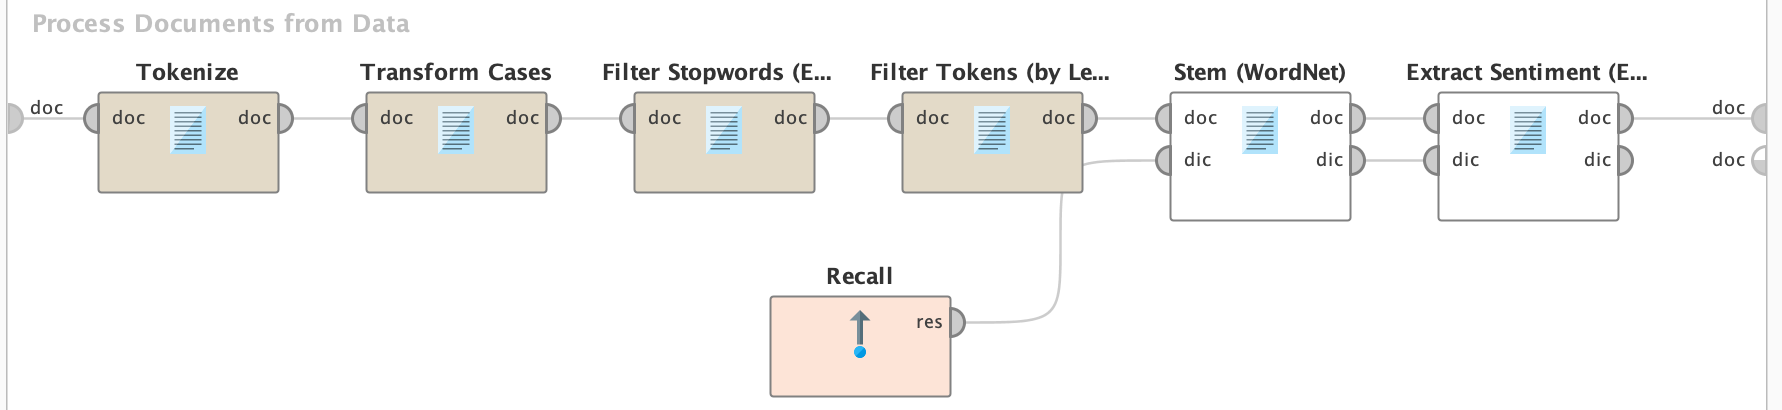
\includegraphics[width=\linewidth]{imgs/part_3/3_processing_documents_full}
	\caption{Process Documents from Data with all elements}
	\label{fig:3_processing_documents_full}
\end{figure}

\begin{figure}[H]
    \centering
    \begin{subfigure}[b]{0.3\textwidth}
        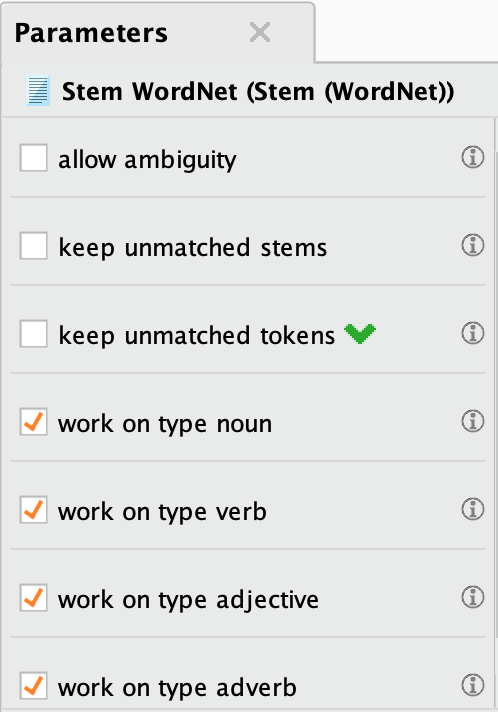
\includegraphics[width=\textwidth]{imgs/part_3/3_processing_documents_stem_wordnet_params_default}
        \caption{Default parameters from the stem via WordNet}
        \label{fig:3_processing_documents_stem_wordnet_params_default}
    \end{subfigure}
    \hspace{0.1\textwidth}
    \begin{subfigure}[b]{0.3\textwidth}
        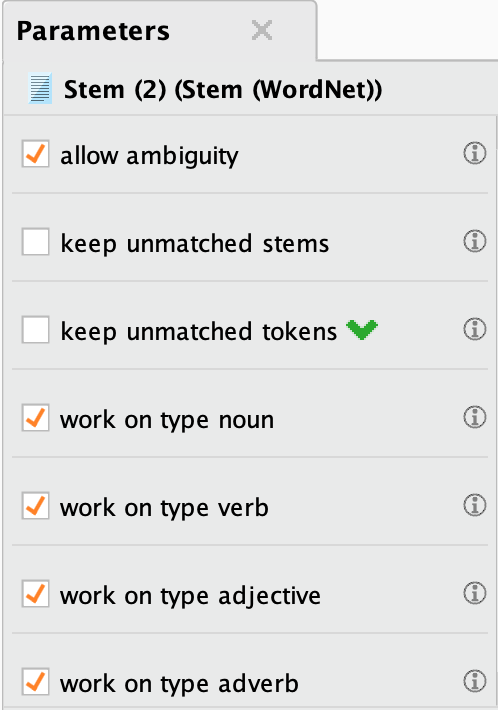
\includegraphics[width=\textwidth]{imgs/part_3/3_processing_documents_stem_wordnet_params_best}
        \caption{Best parameters from the stem via WordNet}
        \label{fig:3_processing_documents_stem_wordnet_params_best}
    \end{subfigure}
    \caption{Parameters from the stemming via WordNet}
    \label{fig:3_processing_documents_stem_wordnet_params}
\end{figure}
\begin{figure}[H]
	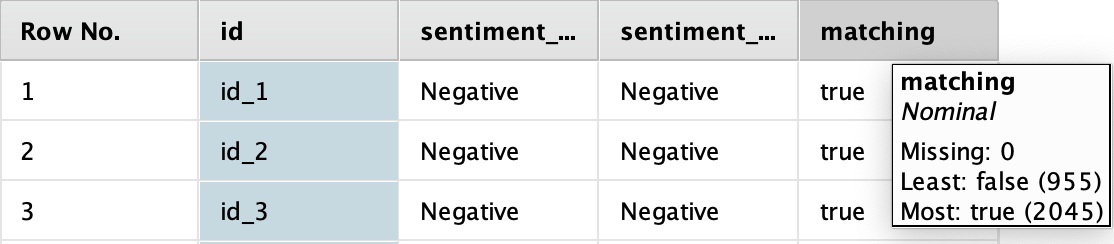
\includegraphics[width=\linewidth]{imgs/part_3/3_processing_documents_with_stem_wordnet_results}
	\caption{Results on using the default WordNet stemming parameters}
	\label{fig:3_processing_documents_with_stem_wordnet_results}
\end{figure}
\begin{figure}[H]
	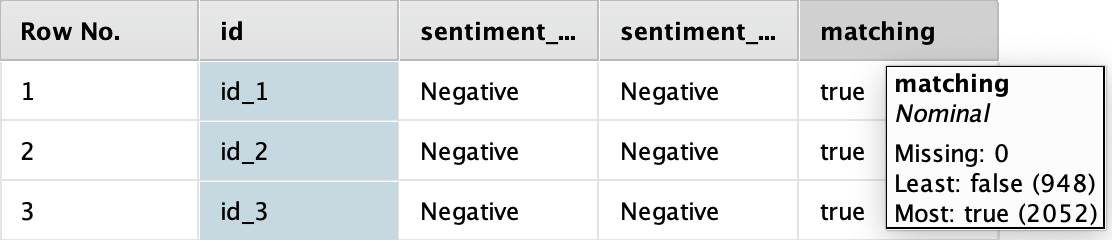
\includegraphics[width=\linewidth]{imgs/part_3/3_processing_documents_with_stem_wordnet_best_results}
	\caption{Results on using the best WordNet stemming parameters}
	\label{fig:3_processing_documents_with_stem_wordnet_best_results}
\end{figure}


\vspace{6pt}
\subsubsection{Modification du module d'extraction de sentiment}
Il nous reste, à présent, plus que le module d'extraction de sentiment à customiser. En effet, jusqu'à présent nous avons utilisé sa configuration par défaut (Fig.\ref{fig:3_processing_documents_full_0_05}), qui nous a permis d'obtenir performance cumulée de \textbf{68.4\%} (Fig.\ref{fig:3_processing_documents_stem_wordnet_params_best}). En jouant avec les paramètres à disposition(Fig.{\ref{fig:3_processing_documents_full_0_001}) nous avons réussit à obtenir une performance de \textbf{70.4\%}.(Fig.\ref{fig:3_processing_documents_full_best_results})

\begin{figure}[H]
\centering
	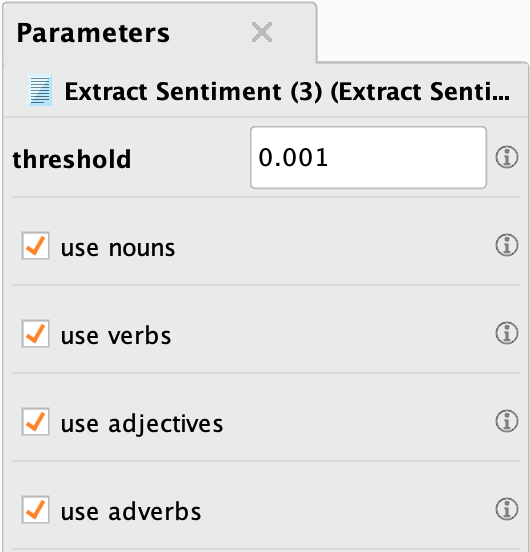
\includegraphics[width=\linewidth/3]{imgs/part_3/3_processing_documents_full_0_001}
	\caption{Extract Sentiment with threshold at 0.001}
	\label{fig:3_processing_documents_full_0_001}
\end{figure}
\begin{figure}[H]
	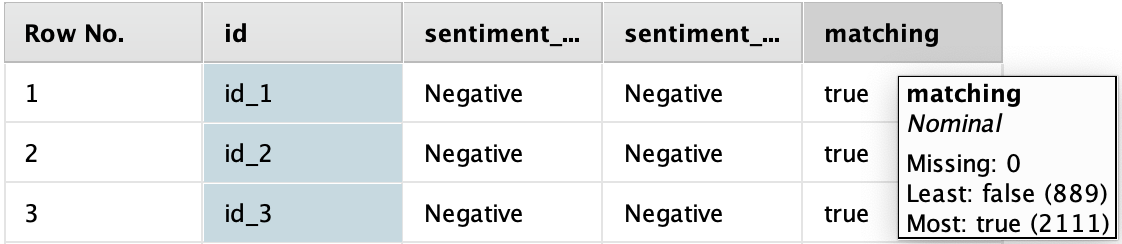
\includegraphics[width=\linewidth]{imgs/part_3/3_processing_documents_full_best_results}
	\caption{Results on using the best WordNet stemming parameters}
	\label{fig:3_processing_documents_full_best_results}
\end{figure}

\vspace{6pt}
\subsection{Notre meilleur modèle de prédiction cumulée}
Nous n'avions qu'un module nous dégradant la prédiction(Fig.\ref{fig:3_processing_documents_no_stem_filter_token}), le filtre de stopwords. Nous l'avons donc supprimée de notre topologie (Fig.\ref{fig:3_processing_documents_optimized}) et terminons avec une performance de \textbf{72.6\%}.(Fig.\ref{fig:3_processing_documents_optimized_best_results})
\begin{figure}[H]
	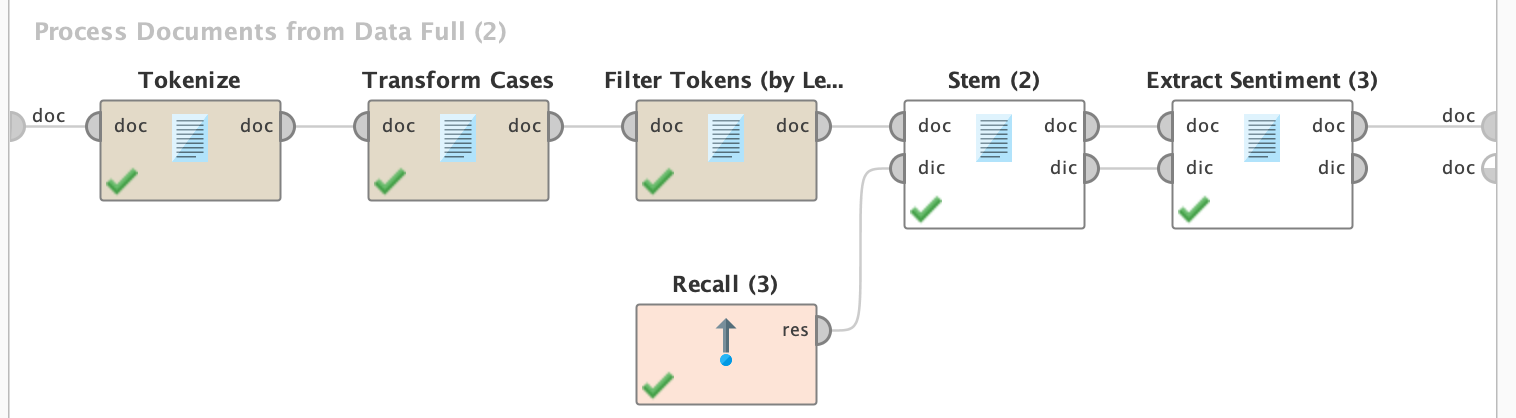
\includegraphics[width=\linewidth]{imgs/part_3/3_processing_documents_optimized}
	\caption{Process Documents from Data with optimized elements}
	\label{fig:3_processing_documents_optimized}
\end{figure}
\begin{figure}[H]
	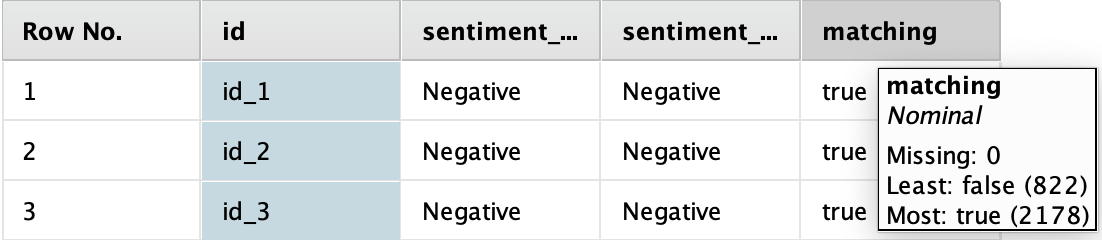
\includegraphics[width=\linewidth]{imgs/part_3/3_processing_documents_optimized_best_results}
	\caption{Results from our best model}
	\label{fig:3_processing_documents_optimized_best_results}
\end{figure}


\section{Conclusion}

\end{document}

%\begin{center}
%	\includegraphics[scale=0.5]{imgs/architecture.png}
%\end{center}

%\begin{lstlisting}[language=sh]
%	$ gradle run
%\end{lstlisting}

%\vspace{6pt}

%\begin{itemize}  
%\item item
%\end{itemize}


%\begin{figure}[H]
%	\includegraphics[width=\linewidth]{imgs/title}
%	\caption{Wikipedia Title}
%	\label{fig:title}
%\end{figure}

